\newpage
\section{Tổng quan Hệ thống}

Chương này mô tả cấu trúc tổng quát của hệ thống giám sát và điều khiển môi trường theo thời gian thực trên ESP32-S3, thiết lập nền tảng lý thuyết trước khi đi vào các giải pháp hiện thực chi tiết. Nội dung tập trung làm rõ kiến trúc phân tầng của hệ thống, tính năng của các thiết bị phần cứng, đồng thời phác thảo mô hình phân rã các tác vụ phần mềm và hạ tầng giao tiếp vận hành (Web Server và Cloud).

\subsection{Kiến trúc phân tầng hệ thống}

Hệ thống được nhóm thiết kế theo mô hình kiến trúc phân tầng tiêu chuẩn của một hệ sinh thái IoT, tích hợp năng lực tính toán biên (Edge Computing) nhằm tối ưu hóa thời gian thực thi và băng thông truyền thông. Kiến trúc tổng thể bao gồm bốn tầng chức năng cốt lõi:

\begin{enumerate}
    \item \textbf{Tầng thu thập dữ liệu:} Chịu trách nhiệm trích xuất các đại lượng vật lý từ môi trường thực tế. Phân tầng này sử dụng các cảm biến để thu thập thông số môi trường (nhiệt độ, độ ẩm tương đối) và phát hiện các biến động không gian (sự kiện chuyển động).
    \item \textbf{Tầng xử lý biên:} Đóng vai trò là hạt nhân điều phối trung tâm. Vi điều khiển xử lý tín hiệu số, vận hành hệ điều hành thời gian thực để lập lịch đa nhiệm, đồng thời trực tiếp thực thi mô hình trí tuệ nhân tạo thu gọn (TinyML) nhằm suy luận trạng thái cục bộ mà không phụ thuộc vào điện toán đám mây.
    \item \textbf{Tầng chấp hành và trực quan hóa cục bộ:} Chuyển đổi các quyết định điều khiển thành các phản hồi vật lý hoặc tín hiệu hiển thị tại chỗ, bao gồm màn hình ký tự, hệ thống phát xạ LED (đơn sắc và ma trận màu RGB) và cơ cấu động cơ băm xung.
    \item \textbf{Tầng mạng và đám mây:} Đảm nhiệm vai trò thiết lập kênh truyền thông hai chiều. Phân tầng này vừa cung cấp giao diện quản trị cục bộ qua sóng Wi-Fi nội bộ, vừa đồng bộ các bản tin dữ liệu lên nền tảng đám mây CoreIOT theo mô hình xuất bản/đăng ký (Publish/Subscribe).
\end{enumerate}

\subsection{Thành phần cấu trúc phần cứng}

Hệ thống vật lý được cấu thành từ các module phần cứng chuyên biệt, được nhóm lựa chọn nhằm đáp ứng các ràng buộc về dòng dòng tiêu thụ, chuẩn giao tiếp và năng lực xử lý thuật toán:

\subsubsection*{1. Vi điều khiển trung tâm YoloUNO (Tích hợp ESP32-S3)}
Đây là trung tâm tính toán của toàn hệ thống. Sở hữu vi xử lý lõi kép Xtensa LX7 với tần số xung nhịp lên tới 240 MHz, tích hợp tăng tốc phần cứng cho các phép toán vector (phục vụ TinyML), module này đảm nhận việc quản lý bộ nhớ dùng chung, duy trì các kết nối mạng đồng thời (AP và STA mode) và thực thi cơ chế lập lịch đa nhiệm FreeRTOS.

\begin{figure}[h!]
\begin{center}
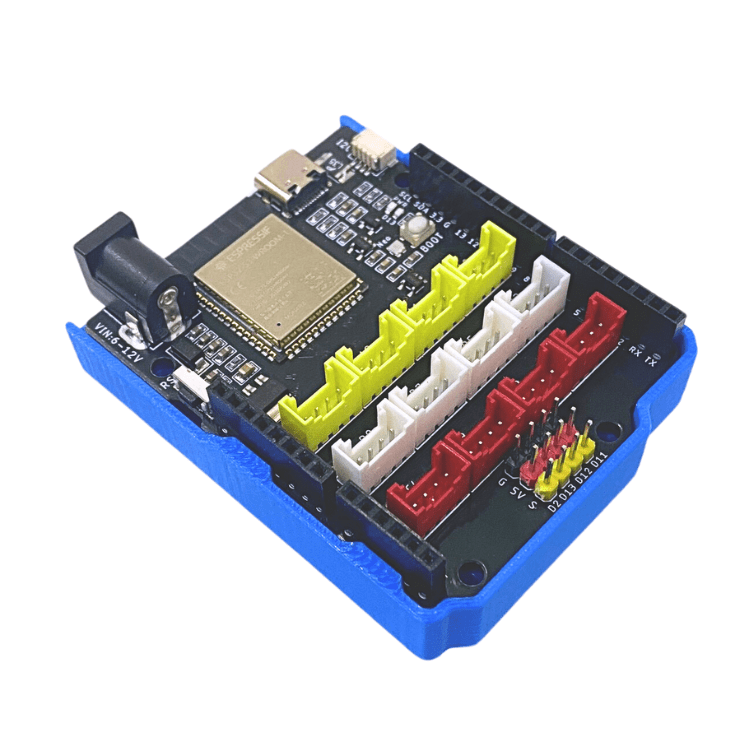
\includegraphics[width=8cm]{pictures/yolo_uno.png}
\end{center}
\caption{Mạch vi điều khiển trung tâm YoloUNO dựa trên kiến trúc ESP32-S3}
\end{figure}

\subsubsection*{2. Cảm biến đo lường nhiệt độ và độ ẩm kỹ thuật số DHT20}
Thiết bị thực hiện nhiệm vụ đo đạc liên tục nhiệt độ và độ ẩm tương đối của môi trường xung quanh. Thiết bị này giao tiếp với vi điều khiển trung tâm thông qua bus I2C ổn định, cung cấp dữ liệu số hóa chính xác, đóng vai trò là nguồn tài nguyên đầu vào cho các tác vụ hiển thị và xử lý logic.

\begin{figure}[h!]
\begin{center}
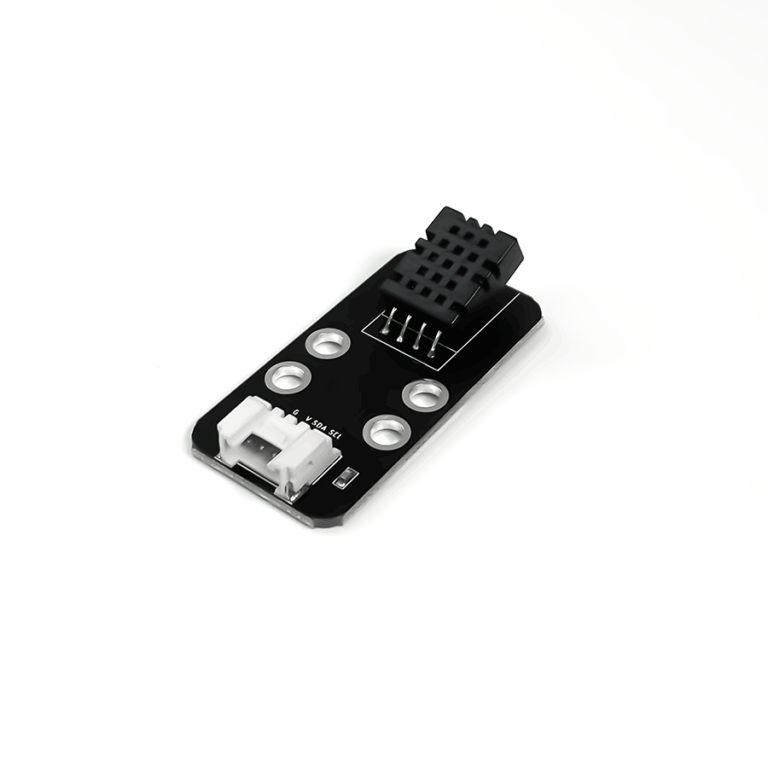
\includegraphics[width=5cm]{pictures/dht20.png}
\end{center}
\caption{Cảm biến đo lường nhiệt độ và độ ẩm kỹ thuật số DHT20}
\end{figure}

\subsubsection*{3. Màn hình LCD 1602 I2C}
Để thực hiện nhiệm vụ hiển thị trực quan thông số đo được từ cảm biến và các thông điệp cảnh báo tại chỗ cho người vận hành, nhóm sử dụng màn hình hiển thị ký tự chuyên dụng LCD 1602. Thiết bị sở hữu khả năng hiển thị cấu trúc định dạng gồm 2 dòng, với mật độ 16 ký tự trên mỗi dòng dựa trên bộ xử lý ma trận điểm và chip điều khiển panel gốc chuẩn công nghiệp HD44780. Linh kiện này được đánh giá cao nhờ độ bền cơ học cao, tính phổ biến trong công nghiệp nhúng và khả năng hỗ trợ thư viện phần mềm tối ưu.

Đặc biệt, để tối ưu hóa tài nguyên phần cứng, màn hình được tích hợp sẵn module chuyển đổi giao tiếp I2C dựa trên chip mở rộng ngoại vi PCF8574. Giải pháp này cho phép nhóm thu gọn toàn bộ luồng truyền tín hiệu song song từ 16 chân kết nối truyền thống xuống còn 2 đường dây dữ liệu số hóa (SDA và SCL) trên bus I2C của vi điều khiển. Sự cải tiến kiến trúc này giúp tiến trình thiết kế mạch diễn ra nhanh chóng, giảm thiểu tối đa sai số phần cứng và giải phóng không gian chân GPIO cho các tác vụ điều khiển động cơ và hệ thống LED.

\begin{figure}[h!]
\begin{center}
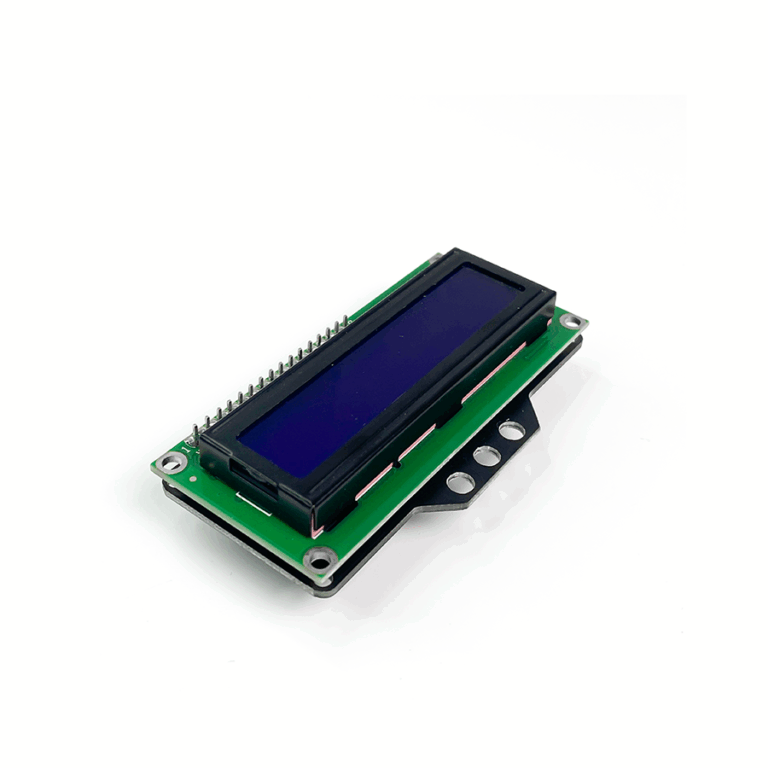
\includegraphics[width=8cm]{pictures/LCD_1602.png}
\end{center}
\caption{Màn hình hiển thị ký tự LCD 1602 với module chuyển đổi I2C}
\end{figure}

\subsubsection*{4. Các module phát xạ ánh sáng cảnh báo (LED tích hợp và LED RGB NeoPixel)}
Hệ thống hiển thị ánh sáng được phân tách thành hai nhiệm vụ: một đèn LED đơn sắc (GPIO 48) chịu trách nhiệm phát tín hiệu xung (Blinking) cảnh báo mức độ nguy hiểm của nhiệt độ, và một đèn LED RGB NeoPixel (GPIO 45) thực hiện ánh xạ dải màu sắc trực quan hóa trạng thái độ ẩm không khí.

\begin{figure}[h!]
\begin{center}
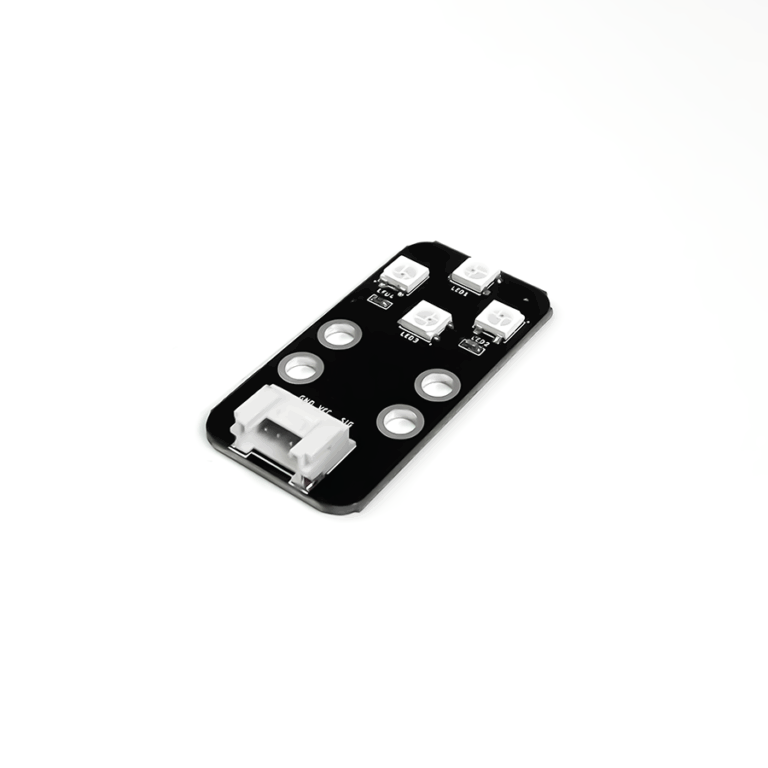
\includegraphics[width=5cm]{pictures/led_RGB.png}
\end{center}
\caption{Cấu trúc module LED RGB đa màu sắc NeoPixel (WS2812B)}
\end{figure}

\subsubsection*{5. Quạt thông gió Mini 5V}
Nhóm sử dụng thiết bị này như một phần mở rộng cho hệ thống, đóng vai trò hạ nhiệt hoặc lưu thông không khí. Động cơ quạt được điều khiển công suất động thông qua kỹ thuật điều chế độ rộng xung (PWM), cho phép thay đổi tốc độ linh hoạt theo yêu cầu điều khiển từ giao diện người dùng.

\begin{figure}[h!]
\begin{center}
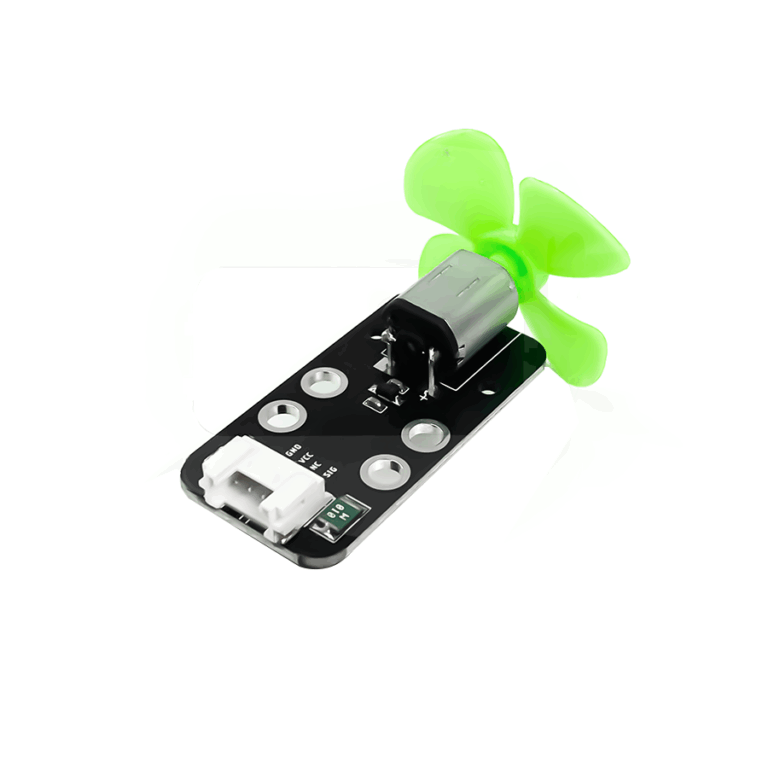
\includegraphics[width=5cm]{pictures/minifan.png}
\end{center}
\caption{Cơ cấu chấp hành Quạt Mini 5V tích hợp mạch đệm công suất}
\end{figure}

\newpage
\subsubsection*{6. Cảm biến hồng ngoại thụ động PIR}
Nằm trong kịch bản mở rộng liên kết mạng thiết bị, cảm biến PIR đóng vai trò phát hiện sự hiện diện của thực thể sống trong không gian giám sát thông qua bức xạ hồng ngoại, kích hoạt các kịch bản báo động an ninh phân tán giữa các node mạng thông qua MQTT Broker nội bộ.

\begin{figure}[h!]
\begin{center}
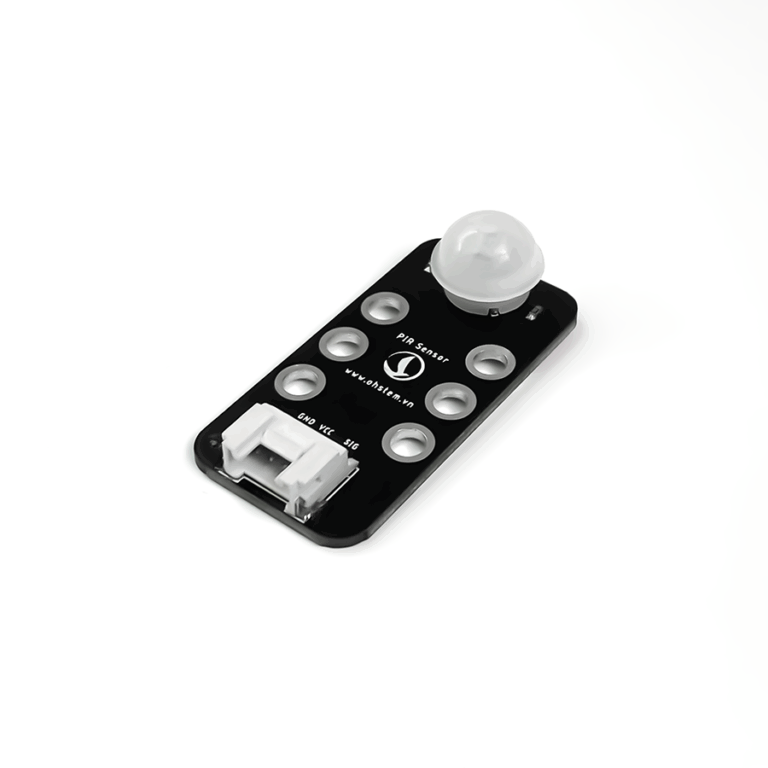
\includegraphics[width=5cm]{pictures/pir.png}
\end{center}
\caption{Cảm biến phát hiện chuyển động hồng ngoại thụ động PIR}
\end{figure}

% \newpage
\subsubsection*{7. Vi điều khiển ESP32-S3-Devkit-C1 N16R8}
ESP32-S3-Devkit-C1 N16R8 được sử dụng như một node phụ trong kiến trúc mở rộng hai thiết bị của hệ thống. Nhờ dùng cùng họ vi điều khiển ESP32-S3, board này tương thích tốt với môi trường PlatformIO, thư viện mạng và mô hình đa nhiệm FreeRTOS đang áp dụng trên node chính. Trong bài toán mở rộng, node Devkit-C1 đảm nhiệm vai trò nhận sự kiện chuyển động từ broker MQTT cục bộ và điều khiển cơ cấu còi báo động theo thời gian thực.

\begin{figure}[h!]
\begin{center}
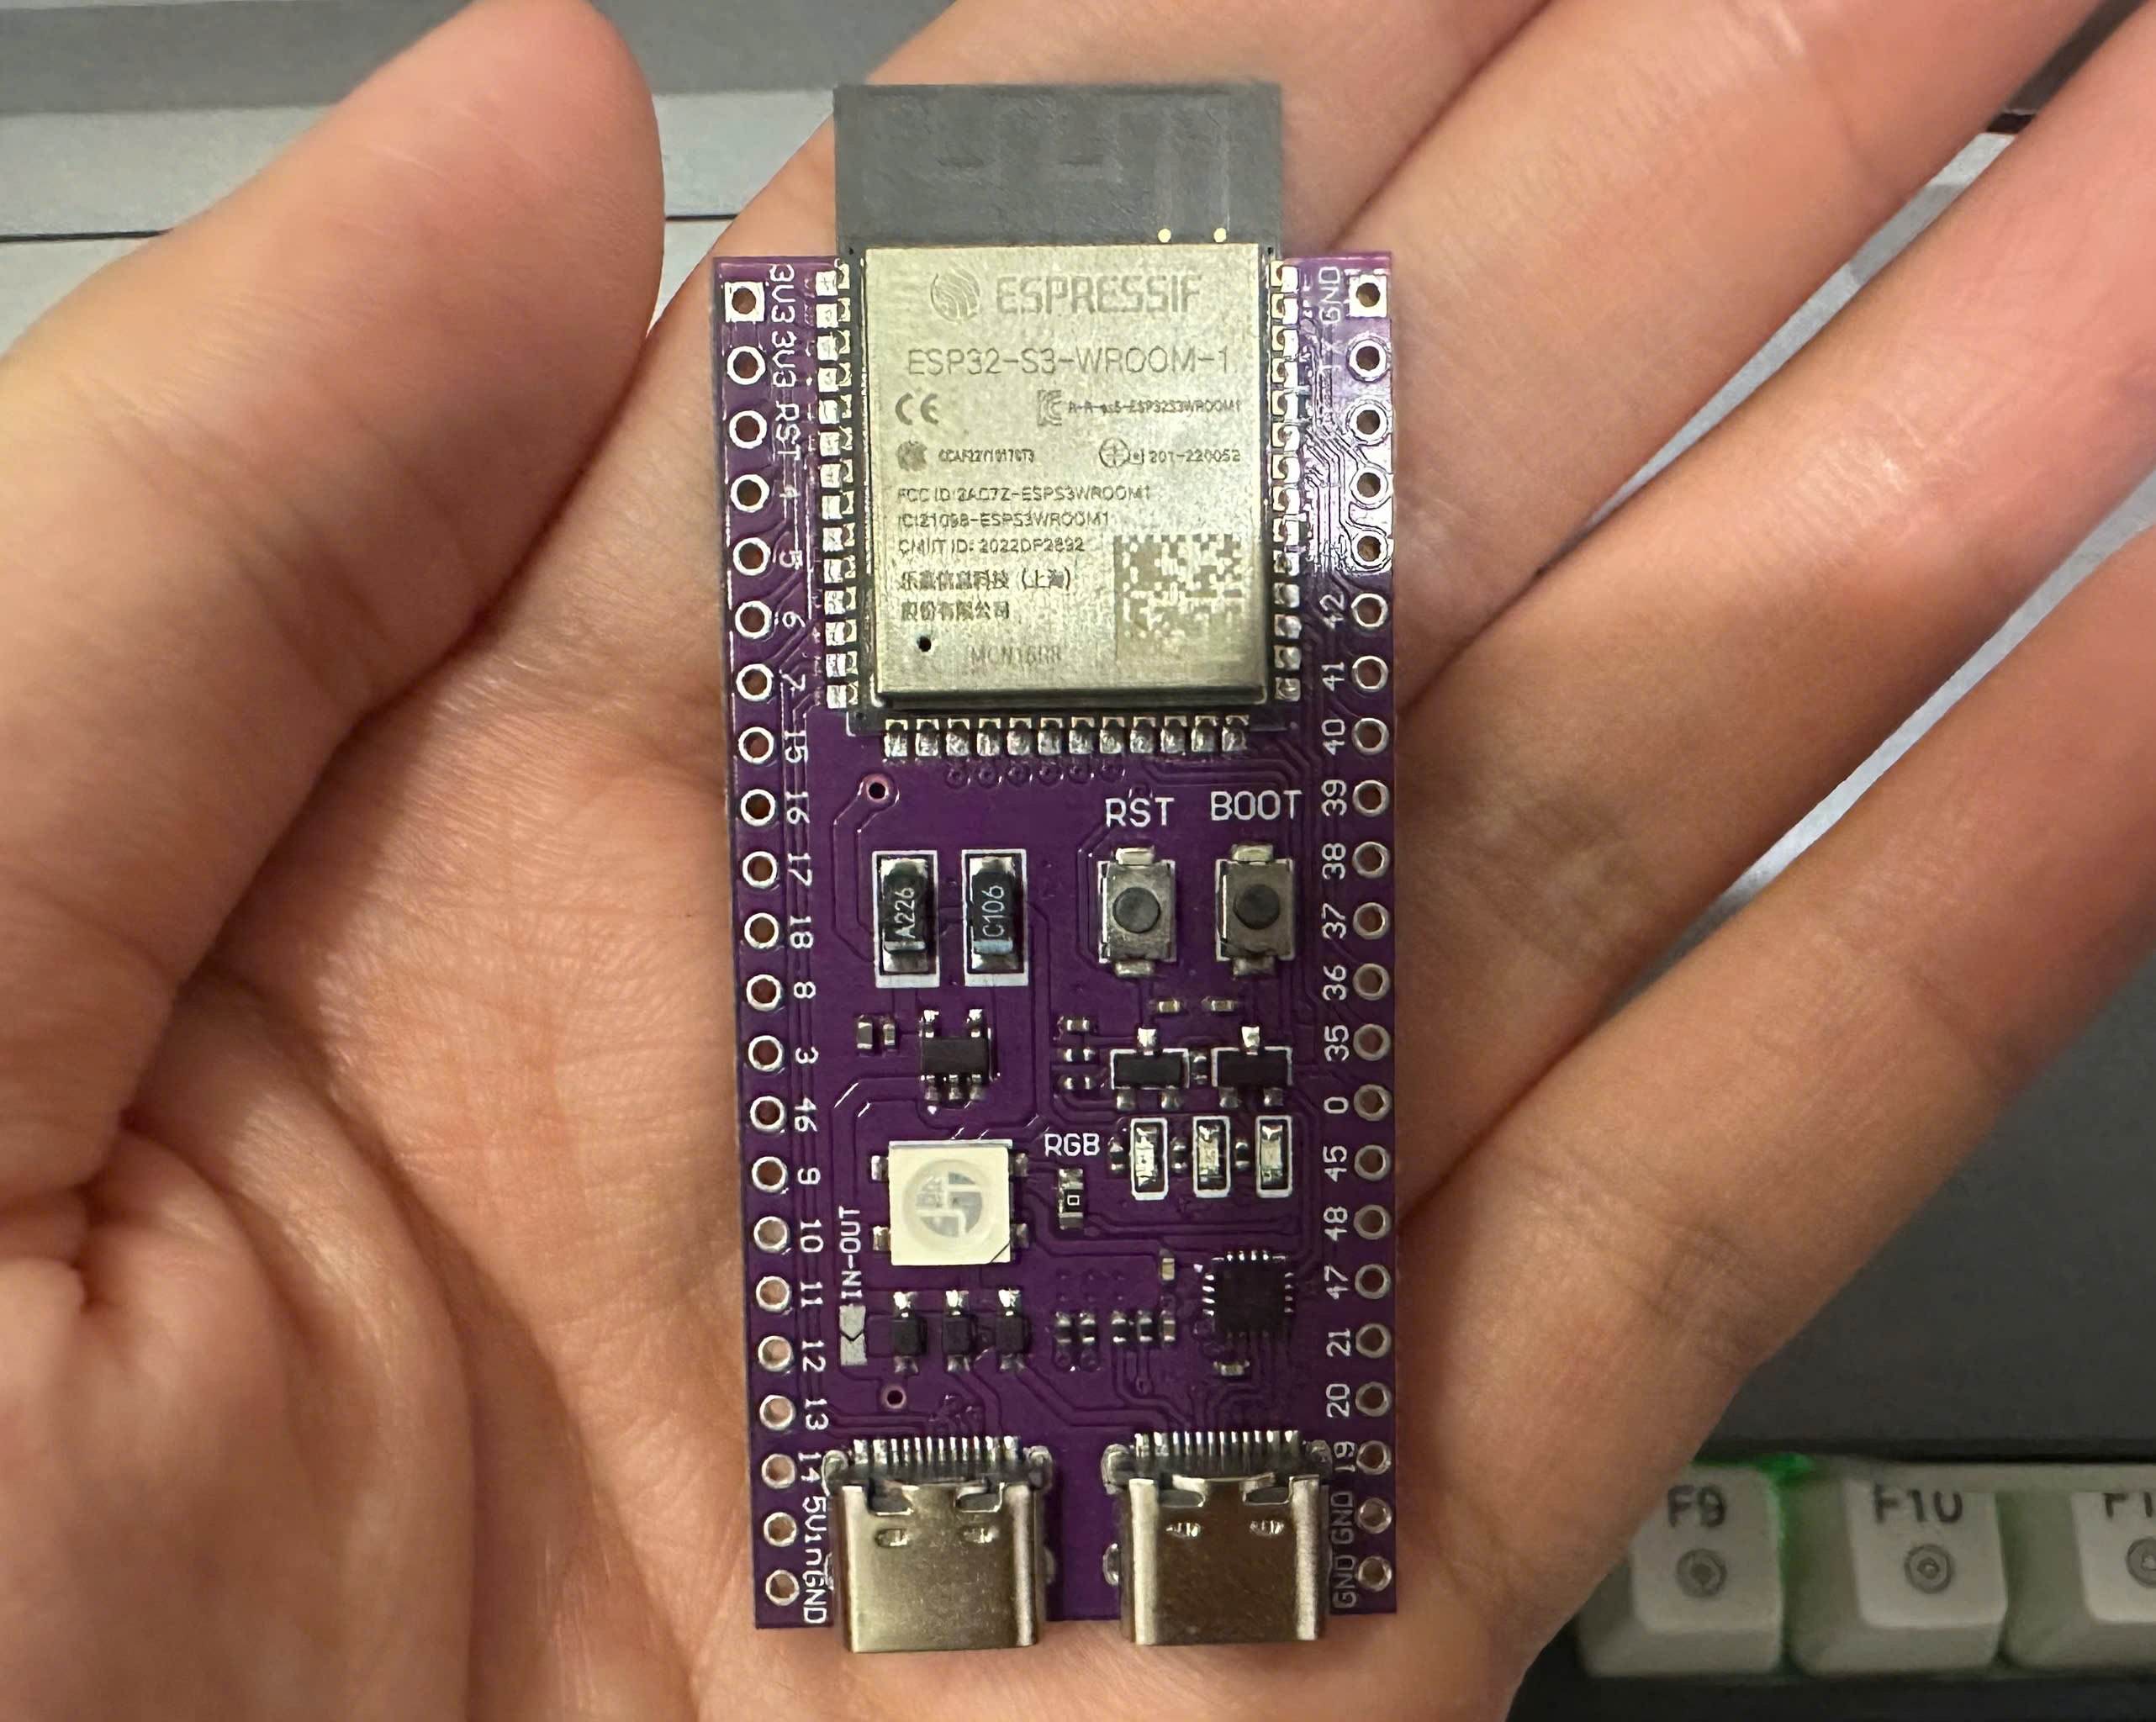
\includegraphics[width=5cm]{pictures/devkitc1.png}
\end{center}
\caption{ESP32-S3-Devkit-C1 N16R8}
\end{figure}

\subsubsection*{8. Còi báo hiệu Buzzer 5V}
Module buzzer 5V là phần tử chấp hành âm thanh dùng để phát cảnh báo khi hệ thống phát hiện chuyển động. Buzzer được kích hoạt bởi node ESP32-S3-Devkit-C1 thông qua tín hiệu điều khiển từ sự kiện MQTT, giúp tách biệt chức năng cảm biến và cảnh báo thành hai thiết bị độc lập. Để đảm bảo an toàn phần cứng, buzzer cần được điều khiển qua tầng đệm công suất (transistor hoặc MOSFET) và sử dụng nguồn 5V ngoài có nối mass chung với vi điều khiển.

\begin{figure}[h!]
\begin{center}
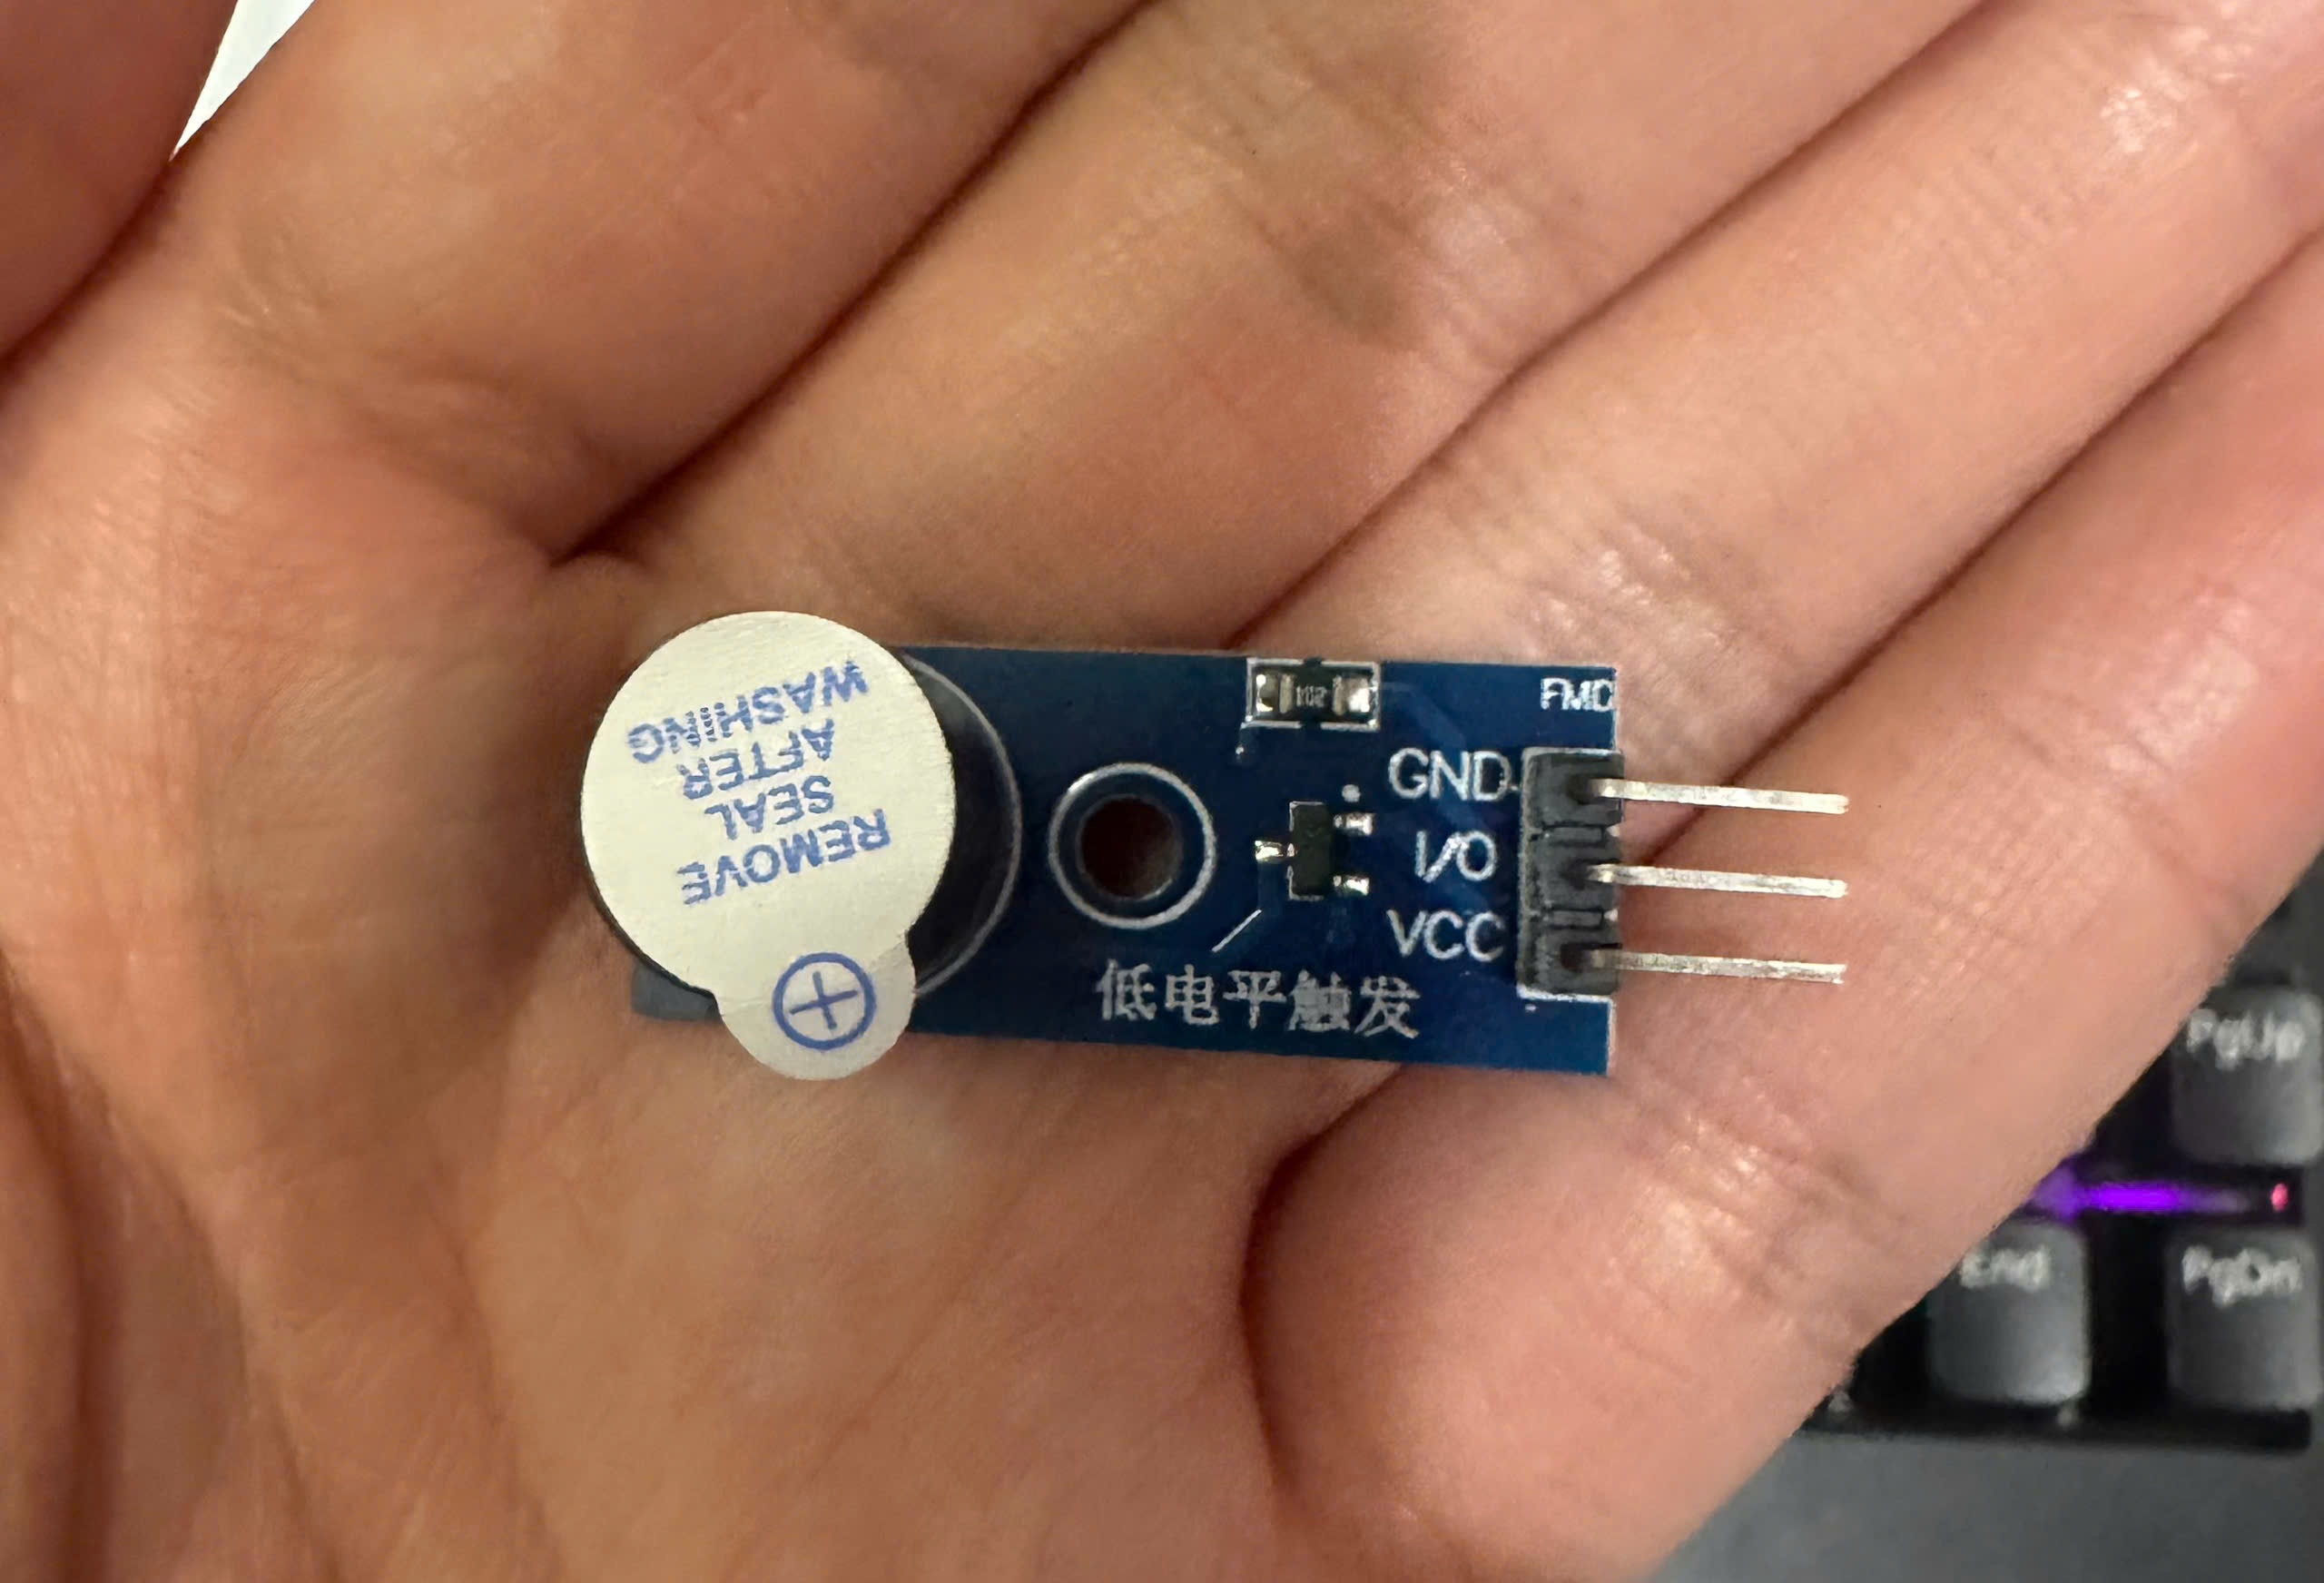
\includegraphics[width=5cm]{pictures/buzzer.png}
\end{center}
\caption{Buzzer 5V}
\end{figure}

\subsection{Kiến trúc phần mềm FreeRTOS và Giao diện vận hành}

Để quản lý tối ưu tính đồng thời của các tác vụ ngoại vi và duy trì các kết nối mạng song song mà không gây nghẽn hệ thống, nhóm triển khai cấu trúc phần mềm dựa trên nền tảng hệ điều hành thời gian thực FreeRTOS. Toàn bộ trạng thái hoạt động của hệ thống được đóng gói tập trung trong cấu trúc cấu trúc dữ liệu dùng chung (\texttt{SharedData}) và được bảo vệ nghiêm ngặt chống xung đột tài nguyên bằng các khóa loại trừ tương hỗ (Mutex).

\paragraph{Mô hình phân rã tác vụ:}
Luồng thực thi của chương trình được chia nhỏ thành các tác vụ chạy song song có kiểm soát chu kỳ độc lập:
\begin{itemize}
    \item Tác vụ thu thập và xử lý biên (\texttt{temp\_humi}, \texttt{tinyMLTask}): Thu thập dữ liệu thô từ phần cứng cảm biến và chạy mô hình mạng nơ-ron suy luận.
    \item Tác vụ hiển thị và thực thi vật lý (\texttt{led\_blinky}, \texttt{controlNeoLED}, \texttt{displayLCD}, \texttt{actuatorTask}): Đáp ứng các sự kiện biến động môi trường để cập nhật trạng thái thiết bị ngoại vi vật lý.
    \item Tác vụ kết nối và giao tiếp mạng (\texttt{webServerTask}, \texttt{WiFi\_connect}, \texttt{CoreIoT\_Task}): Đảm nhiệm duy trì hạ tầng mạng và xử lý các giao thức lớp ứng dụng.
\end{itemize}

\paragraph{Kiến trúc giao diện vận hành hai lớp (Dual-Interface Architecture):}
Giao diện tương tác với người dùng (HMI) được thiết kế phân cấp rõ ràng nhằm tối ưu hóa kịch bản vận hành thực tế. Cả hai nền tảng giao diện đều được tích hợp đầy đủ tính năng giám sát và điều khiển:

\begin{itemize}
    \item \textbf{Giao diện giám sát cục bộ (Local Web Server):} Vận hành trực tiếp trên bộ nhớ vi điều khiển ở chế độ Access Point (AP). Giao diện này được nhóm thiết kế trực quan, chia thành các khối (Card) chức năng rõ ràng nhằm tối ưu hóa trải nghiệm người dùng:
    \begin{itemize}
        \item \textbf{\textit{Khối giám sát (Monitoring):}} Hiển thị nhiệt độ, độ ẩm thời gian thực.
        \item \textbf{\textit{Khối điều khiển (Actuators):}} Tích hợp thanh trượt PWM điều tốc quạt làm mát và bảng điều khiển phối màu R-G-B cho Smart LED.
        \item \textbf{\textit{Thanh trạng thái:}} Cho phép người dùng nhập cấu hình Wi-Fi hạ tầng (SSID/Password).
    \end{itemize}
    Nhờ hạ tầng này, hệ thống vẫn có khả năng được cấu hình và vận hành hoàn toàn bình thường ngay cả khi mất kết nối Internet toàn cục.

    \begin{figure}[h!]
    \begin{center}
    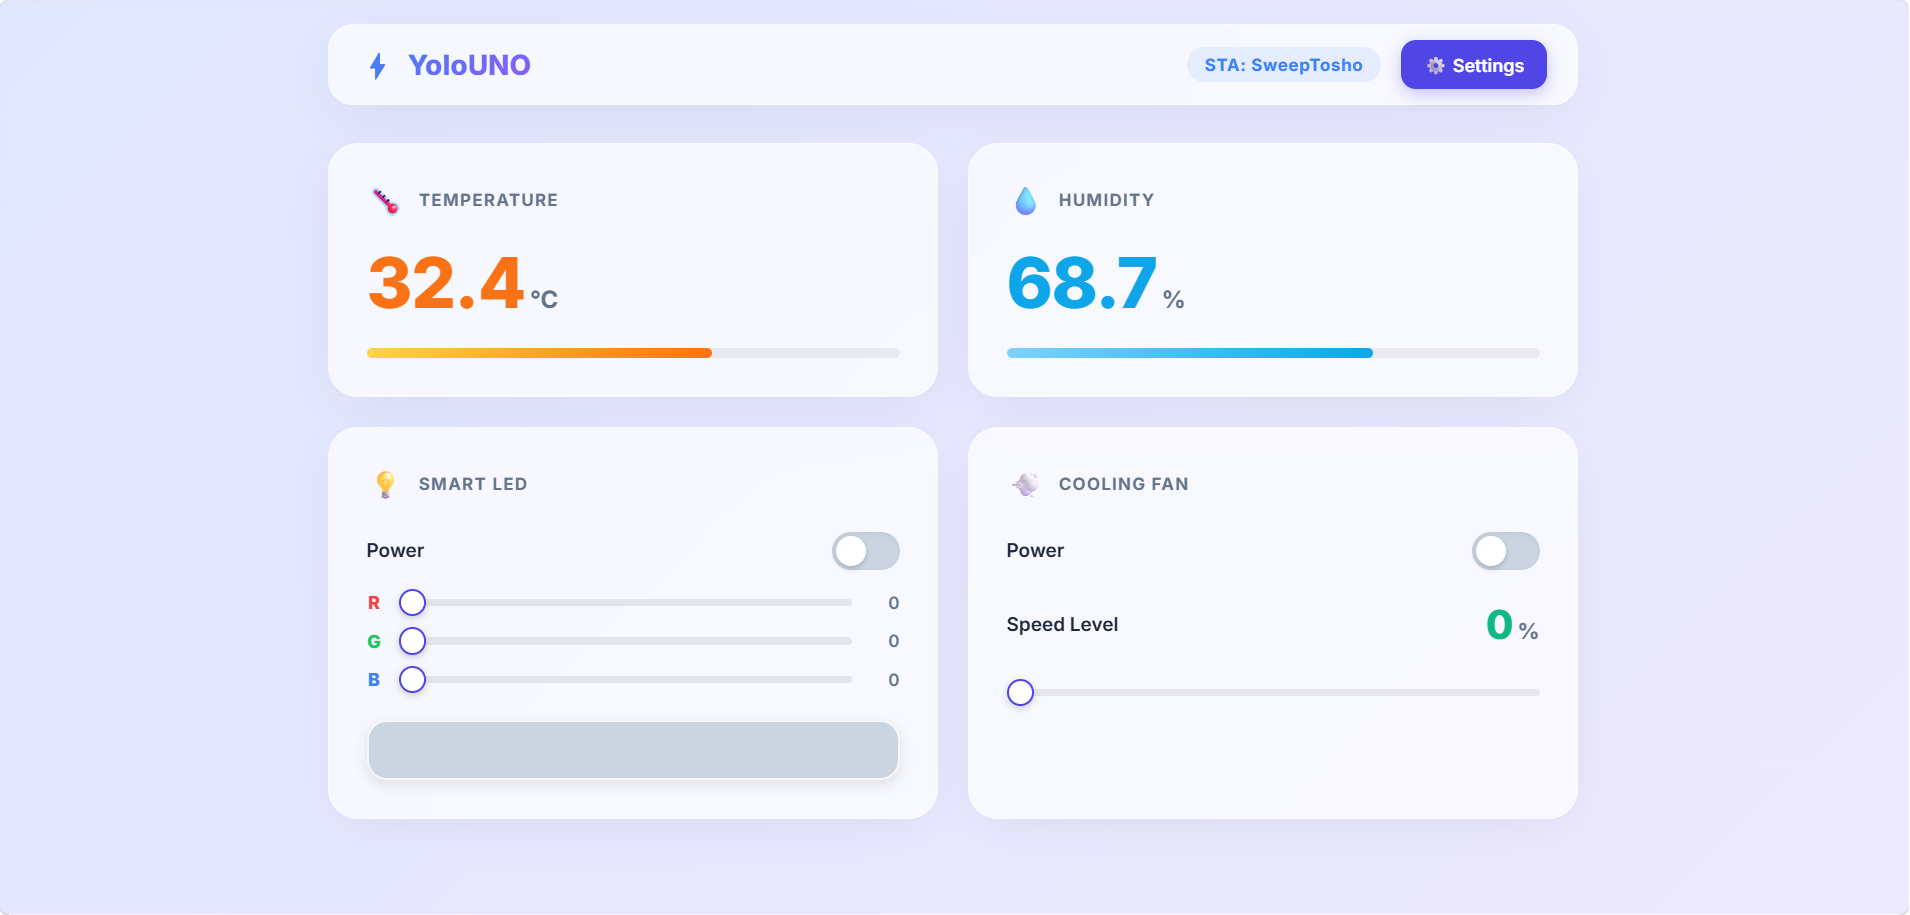
\includegraphics[width=1\textwidth]{pictures/web_server.png}
    \end{center}
    \caption{Giao diện Dashboard điều khiển và giám sát cục bộ trên Web Server}
    \end{figure}

    \item \textbf{Giao diện giám sát đám mây từ xa (CoreIOT Cloud Dashboard):} Hoạt động khi thiết bị đã hòa mạng Internet (STA mode). Tuân thủ đặc tả kỹ thuật của bài tập lớn, nhóm đã tái sử dụng các Template (mẫu giao diện) chuẩn công nghiệp có sẵn trên hệ sinh thái CoreIOT, sau đó tiến hành tùy biến sâu (Customization) để tương thích với kiến trúc của dự án. Dashboard được chia thành hai phân hệ:
    \begin{itemize}
        \item \textbf{\textit{Phân hệ viễn trắc (Telemetry):}} Tùy biến các thẻ số liệu (Digital Gauge) và biểu đồ đường (Line Chart) nhằm lưu trữ và hiển thị xu hướng biến thiên của nhiệt độ, độ ẩm trong quá khứ.
        \item \textbf{\textit{Phân hệ điều khiển Ghi đè (RPC Actuators):}} Tùy biến bổ sung các công tắc dạng gạt (Toggle Switch). Các công tắc này được gán với các luồng RPC (Remote Procedure Call), cho phép người quản trị từ xa kích hoạt chế độ Cưỡng chế ghi đè (Manual Override), ép trạng thái LED thay đổi bất chấp logic cảm biến tự động tại biên.
    \end{itemize}


    \begin{figure}[h!]
    \begin{center}
    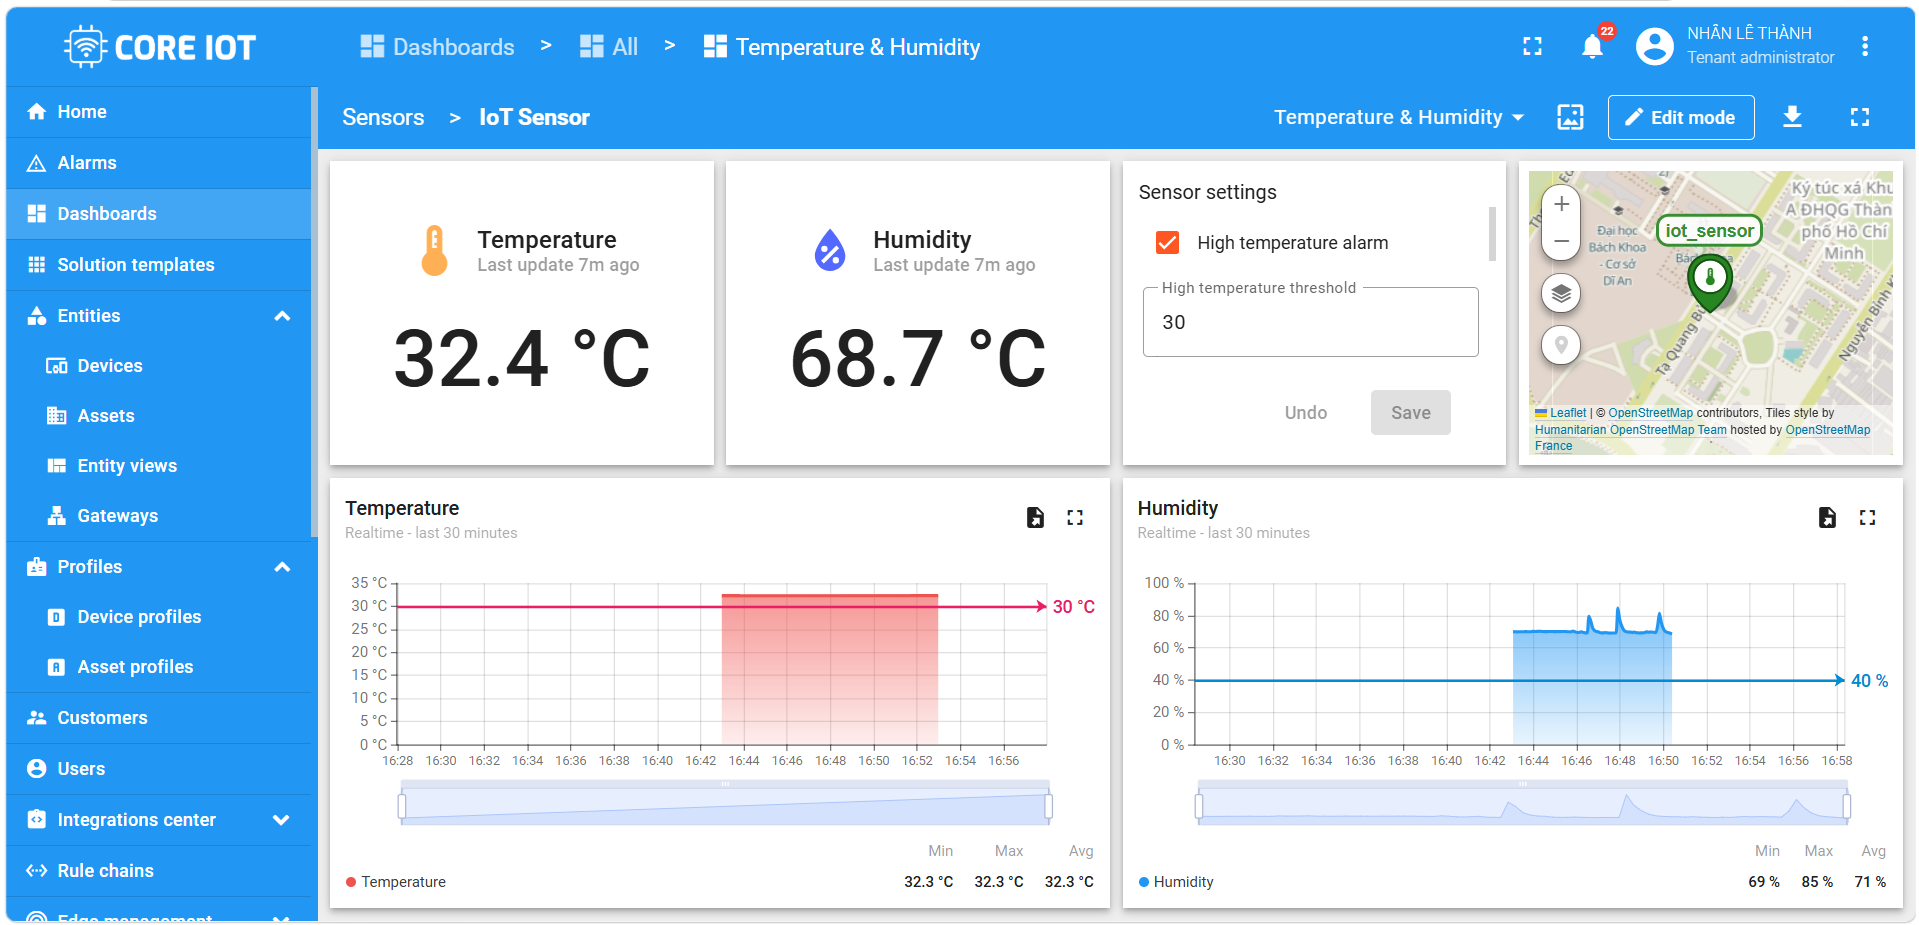
\includegraphics[width=1\textwidth]{pictures/coreiot_dash_main.png}
    \end{center}
    \caption{Giao diện giám sát dữ liệu viễn trắc và bản đồ định vị tùy biến trên nền tảng CoreIOT}
    \end{figure}

    \begin{figure}[h!]
    \begin{center}
    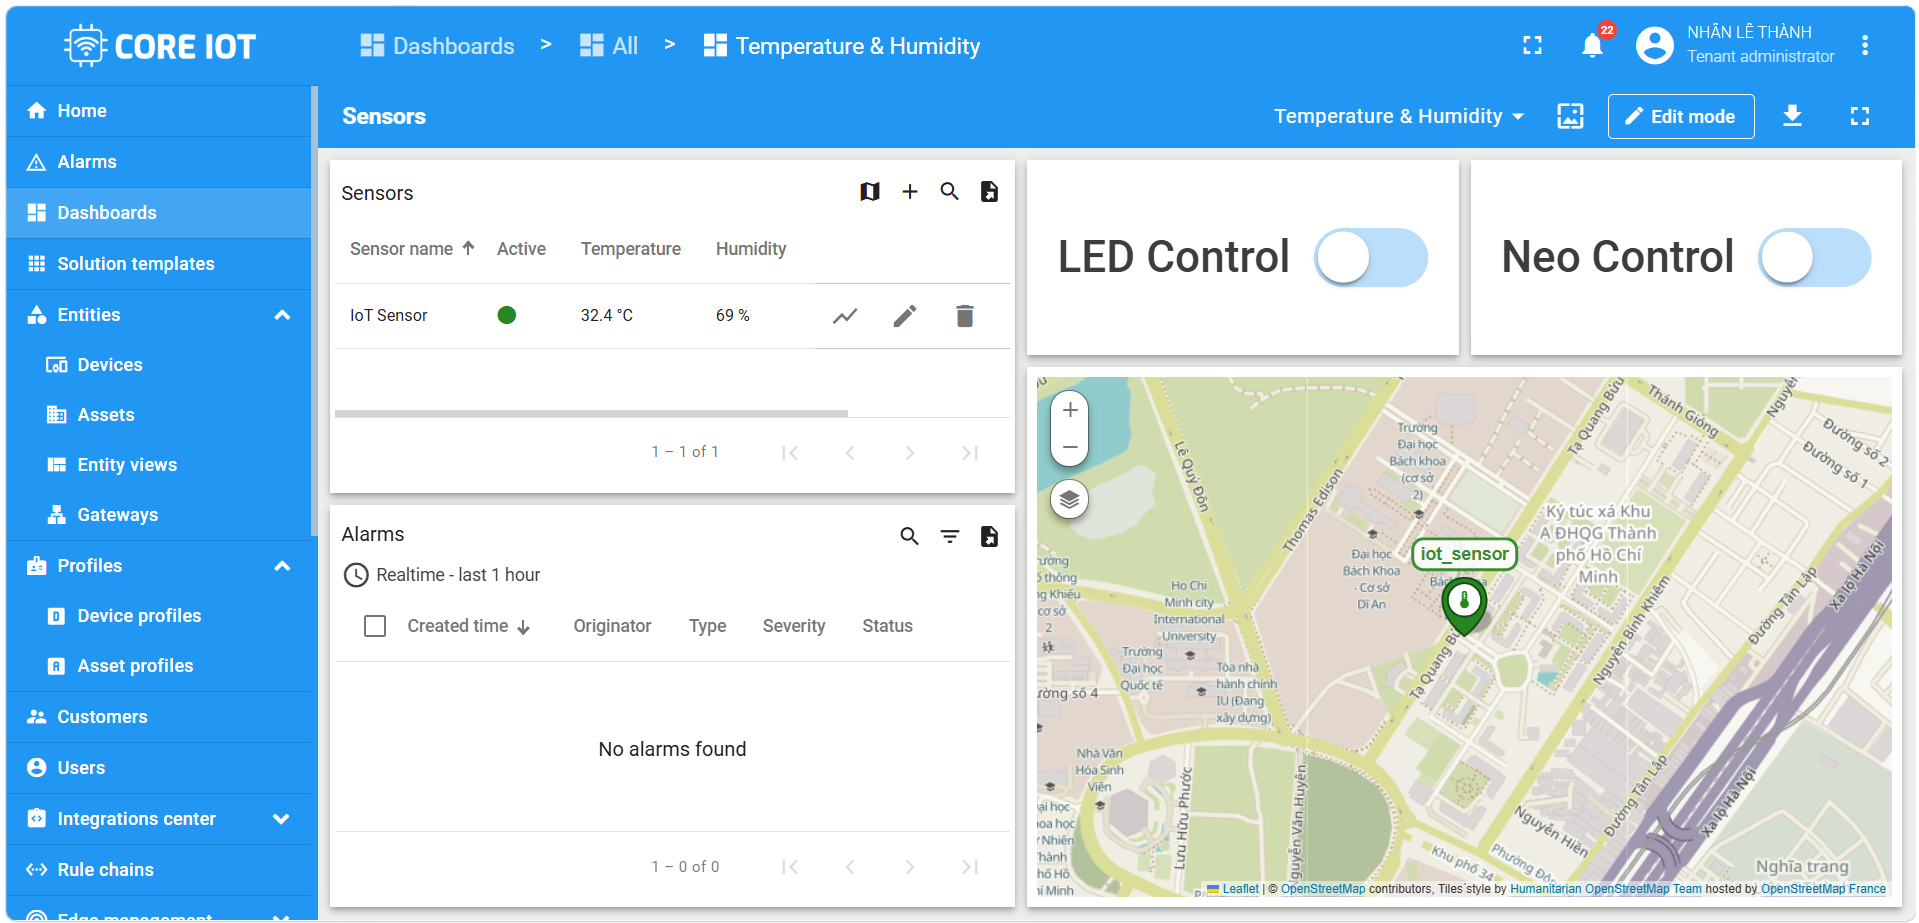
\includegraphics[width=1\textwidth]{pictures/coreiot_dash_rpc.png}
    \end{center}
    \caption{Các Widget Switch RPC được nhóm bổ sung phục vụ cơ chế Manual Override}
    \end{figure}
\end{itemize}

Sự kết hợp đồng bộ giữa giải pháp phần cứng phân tán và kiến trúc phần mềm đa nhiệm, đa giao diện này đảm bảo tính toàn vẹn dữ liệu, loại bỏ các mối đe dọa về xung đột tài nguyên phần cứng và cung cấp một giải pháp IoT toàn diện, sẵn sàng mở rộng quy mô.
